\documentclass[12pt]{report}

% Language setting
% Replace `english' with e.g. `spanish' to change the document language
\usepackage[english]{babel}

% Set page size and margins
% Replace `letterpaper' with `a4paper' for UK/EU standard size
\usepackage[letterpaper,margin=1in,marginparwidth=1.75cm]{geometry}
\geometry{letterpaper}

% Useful packages
\usepackage{amsmath,amsthm,amssymb,color,latexsym,mathtools}
\usepackage{graphicx}
\usepackage{hyperref}
\usepackage{subfig}
\usepackage{mathtools}
\usepackage{booktabs}
\usepackage{cancel}
\usepackage[all]{xy}
\usepackage{cleveref}
\usepackage{csquotes}

\usepackage{bm}

\usepackage[shortlabels]{enumitem}
\usepackage[table]{xcolor}
\usepackage{url}

\usepackage{parskip}

% bibliography
\usepackage[backend=biber]{biblatex}
\addbibresource{citations.bib}

% glossaries
\usepackage[toc]{glossaries}
\loadglsentries{glossary}
\makeglossaries


% \numberwithin{equation}{subsection}

\usepackage{array}
\usepackage{float}
\usepackage[labelfont=bf, font={small,sf}]{caption}
\usepackage{circuitikz}
\usepackage{gensymb}


\setlength{\parindent}{0pt}

% math theorem styles

\newtheorem{problem}{Problem}

\newtheorem{theorem}{Theorem}
\newtheorem*{proposition}{Proposition}
\newtheorem{lemma}[theorem]{Lemma}
\newtheorem{corollary}[theorem]{Corollary}
\newtheorem{conjecture}[theorem]{Conjecture}
\newtheorem{postulate}[theorem]{Postulate}

\theoremstyle{definition}
\newtheorem{defn}[theorem]{Definition}
\newtheorem{example}[theorem]{Example}

\theoremstyle{remark}
\newtheorem*{remark}{Remark}
\newtheorem*{notation}{Notation}
\newtheorem*{note}{Note}
\usepackage{setspace}

\newenvironment{solution}[1][\it{Solution}]{\textbf{#1. } }{$\square$}

\newcommand{\ndiv}{\not\hspace{2.5pt}\mid}

% modify this to change spacing
\setstretch{1}

% figure out subfles or smth later
\usepackage{subfiles}

%%%%%%%%%%%%%%%%%%%%%%%%%%%%%%%%%%%%%%%%%%%%%%%%%%%%%%%%%%%%%

\begin{document}

\title{robot doggo can learn how to walk???}
\author{Sky Hong}
\date{\today}
\maketitle

\begin{abstract}
    something idk, figure out final formatting later
\end{abstract}

%%%%%%%%%%%%%%%%%%%%%%%%%%%%%%%%%%%%%%%%%%%%%%%%%%%%%%%%%%%%%

\tableofcontents
%\addcontentsline{toc}{chapter}{Glossary}

\chapter{Introduction}

\chapter{Background}
\section{Introduction to Machine Learning}
The field of machine learning is fundamentally about finding functions that model data. For example, a speech recognition model takes audio as an input and outputs a text, and AlphaZero takes a chessboard state as an input and outputs a move. These functions may be vastly complex, with far too many parameters and relations for any human to reasonably articulate and program, even if the task comes naturally to our evolved biology. Machine learning offers methods for computers to achieve these tasks, without the need for a human to give explicit instructions on \textit{how} it should be accomplished.

This section will give a very introductory overview of machine learning, the specific details of which will be delved more deeply in following sections. The general framework of creating a machine learning model is as follows:

\begin{enumerate}
    \item Identification of the properties of a model. What should this model be able to do? What are its inputs and outputs? What kind of model architecture is best suited to its problem?
    \item Defining a loss function, some metric to measure how well a model performs.
    \item Optimizing the parameters of a model to minimize the loss function and maximize performance.
\end{enumerate}

\subsection{Parameters}

As an example, consider a simple model consisting of a linear relationship between a data set and the output of the model.
\begin{equation}
    f(\mathbf{x}) = b +\sum_i w_i x_i
\end{equation}

Parameters that directly multiply values, $w_i$, are called \textbf{\glspl{weight}}, and parameters that offset values, $b$, are called \textbf{\glspl{bias}}. The inputs from the data set, $\mathbf{x}$, are called \textbf{\glspl{feature}} This can be generalized to vector outputs with matrices, and in more complex models, the notation may be extended to tensors.
\begin{equation}
    f = \mathbf{b} + W\mathbf{x}
\end{equation}

The parameters of a model are usually collectively referred to as a vector $\boldsymbol{\theta}$, with components of the individual weights and biases of the model. For complex models, $\boldsymbol{\theta}$ may be millions, billions, or even trillions of parameters long, populated by numerous parameter tensors.
\begin{equation}
    \boldsymbol{\theta} = \begin{bmatrix}
        W_{11} \\
        W_{12} \\
        \vdots \\
        b_1 \\
        b_2 \\
        \vdots
    \end{bmatrix}
\end{equation}
For virtually all non-trivial problems, linear relationships are far too reductive to completely capture the complexity of a problem. Such inherent limitations of a model due to its architecture known as \textbf{\gls{model-bias}}. Model architectures will be expounded upon in more detail in Section 1.2.

\subsection{Loss Functions}

A \textbf{\gls{loss-function}} (also sometimes called a \textbf{cost function}), typically denoted $L(\boldsymbol{\theta})$ or just $L$, is the measure of how ``bad'' a set of parameters $\boldsymbol{\theta}$ for a model is. A common definition is the deviation between a model's prediction and an actual result. For example, when building a speech recognition model, the loss may be defined as the error rate between its output transcription and the correct transcription. The features of the training data that are provided to the model, in this case, the correct transcriptions, are identified with \textbf{\glspl{label}} that tell the model what it should train towards.

Losses over all labels in the training data are aggregated into an value for the overall loss function, the most common method of which is the \textbf{\gls{mse}}:
\begin{equation}
    L = \frac{1}{N}\sum (y - \hat{y})^2 .
\end{equation}

$L$ is associated with an \textbf{\gls{error-surface}} that can be understood as the plot of $L$ in a $|\boldsymbol{\theta}|$-dimensional parameter space, though it is usually far too complex to be directly visualized.

\subsection{Optimization}

Since $L$ is continuous, there must exist some set of parameters $\boldsymbol{\theta}^\ast$ that minimize $L$ and model the training data best.
\begin{equation}
    \boldsymbol{\theta}^\ast = \arg\min_{\boldsymbol{\theta}} L
\end{equation}
The process of improving the model by finding values for $\boldsymbol{\theta}$ that lower the loss function is what it really means for a model to ``learn'' or ``train''.

\subsubsection{Gradient descent}

Since brute-forcing the error surface of $L$ is infeasible with a large number of parameters, the standard algorithmic approach to find minima of $L$ is \textbf{gradient descent}. In gradient descent, $L$ is iteratively lowered by stepping $\boldsymbol{\theta}$ against the gradient of $L$.
\begin{equation}
    \boldsymbol{\theta}^{(n+1)} = \boldsymbol{\theta}^{(n)}-\eta\nabla L(\boldsymbol{\theta}^{(n)})
\end{equation}
The \textbf{learning rate}, $\eta$, determines the scaling for the size of each step.

\begin{figure}[h]
    \centering
    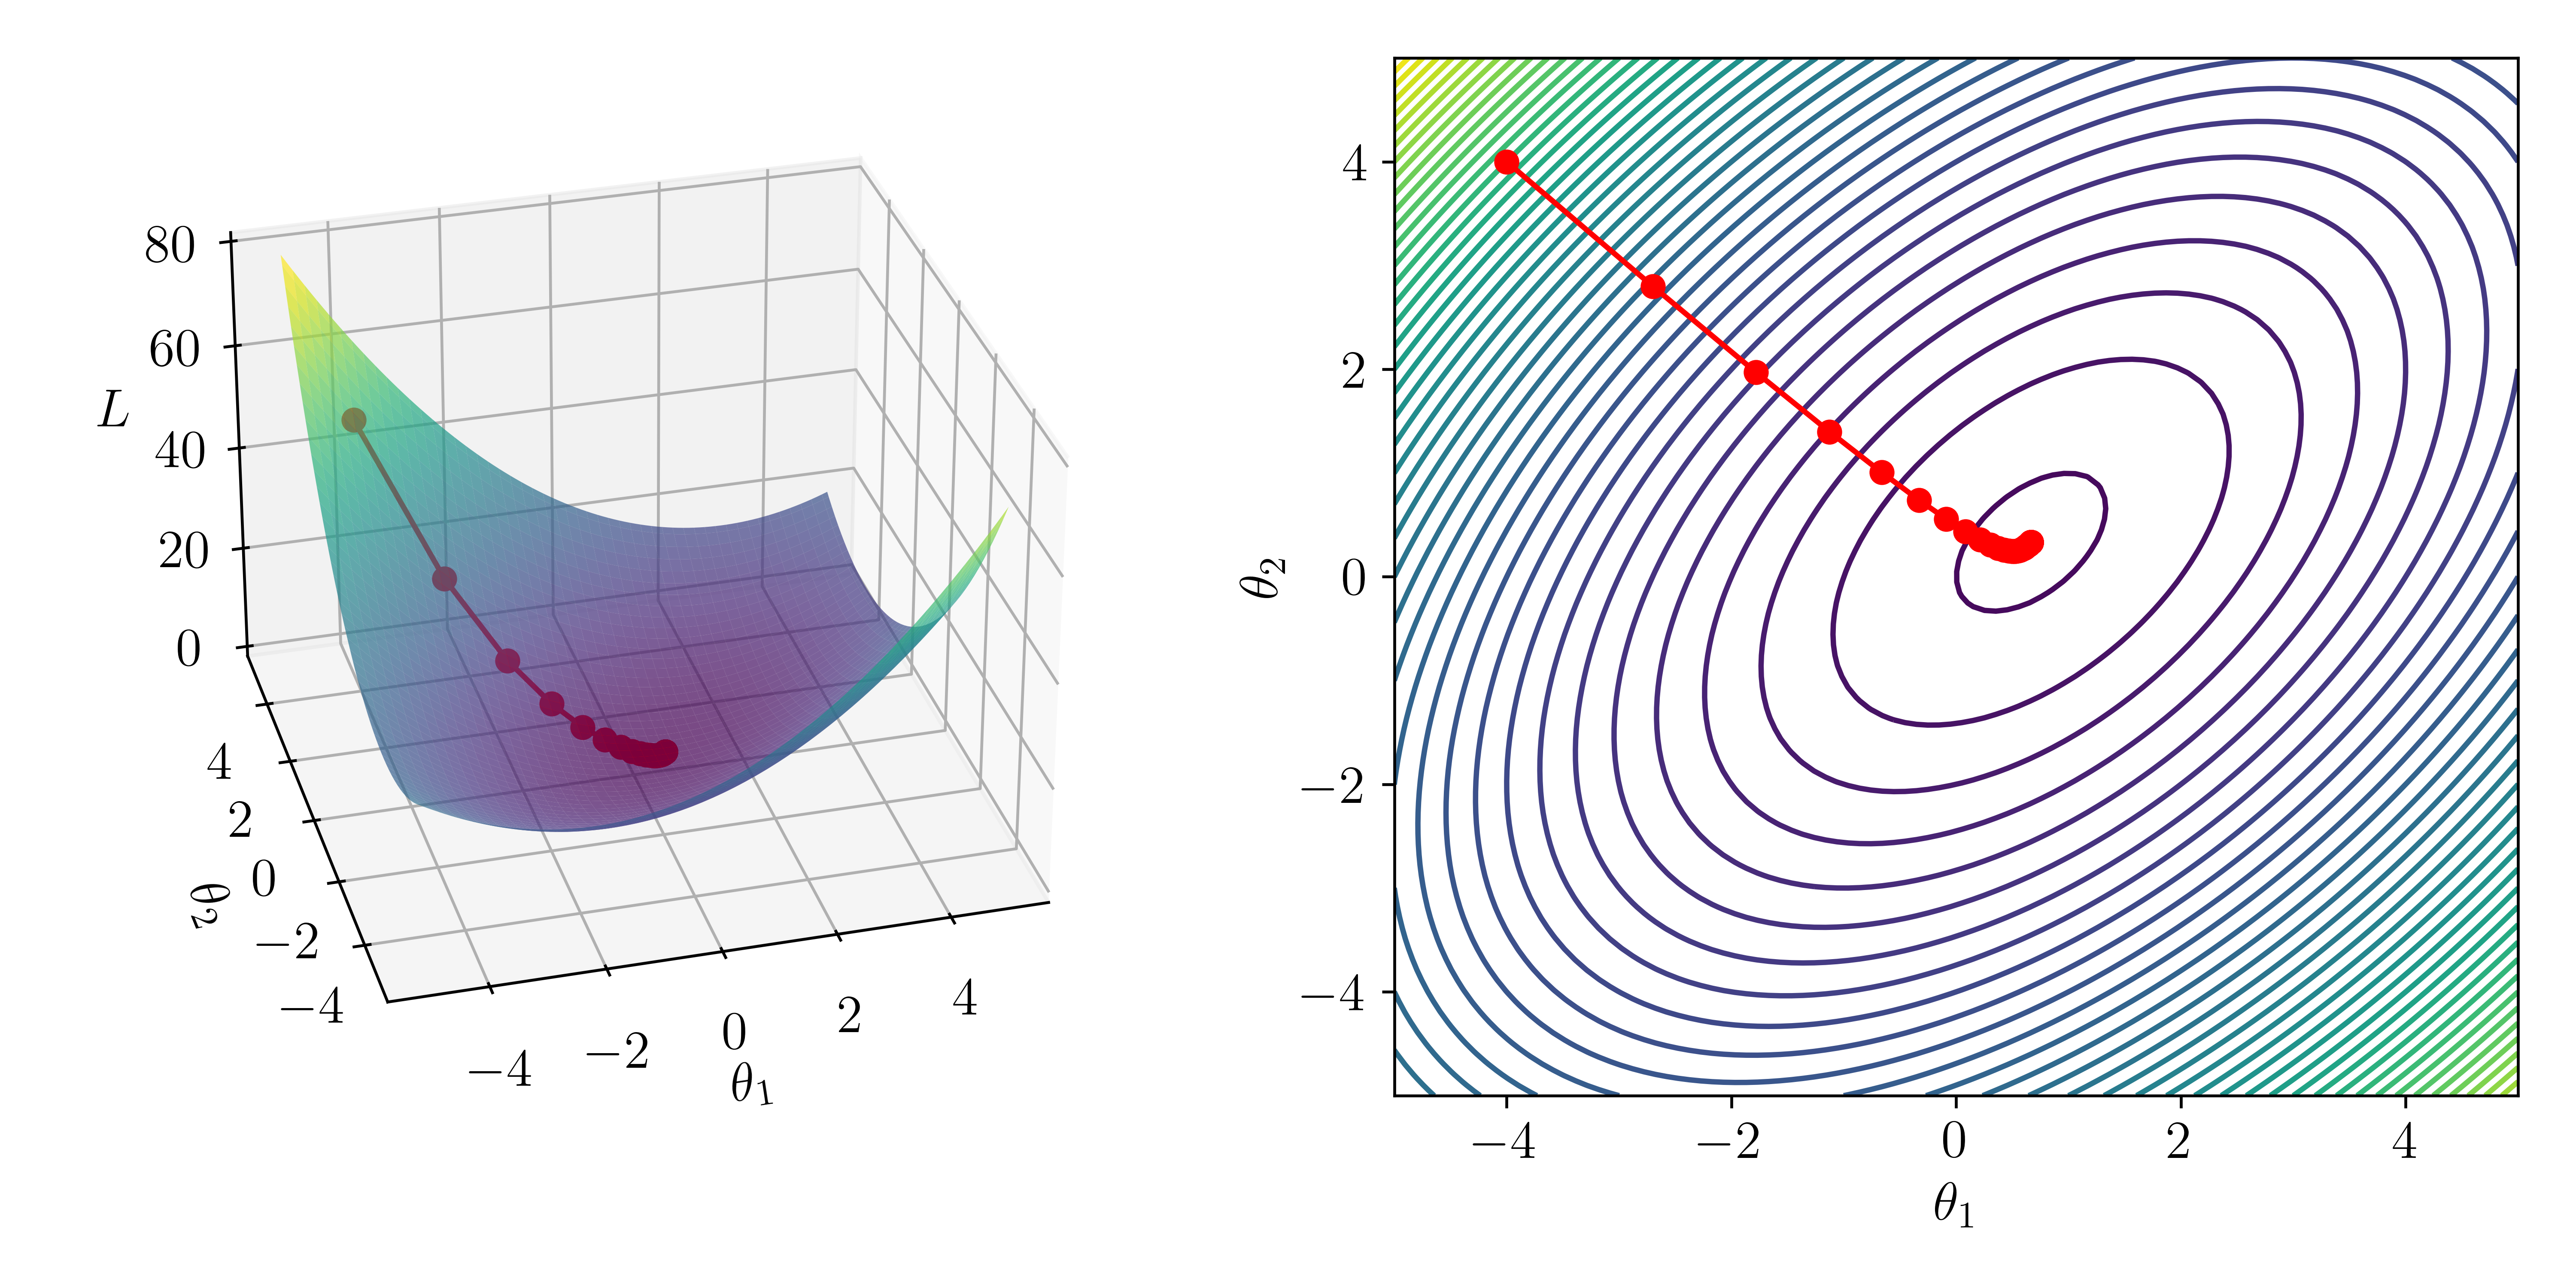
\includegraphics[width=\linewidth]{figs/gradient_descent.png}
    \caption{Visualization of naive gradient descent on an error surface with two parameters ($L = \theta_1^2 + \theta_2^2 - \theta_1\theta_2 - \theta_1$) by a 3D plot (left), and a contour plot (right). The red line shows $100$ iterations of gradient descent, starting from intial parameters $\boldsymbol{\theta}^{(0)} = [-4,4]$, with $\eta = 0.1$. (Original)}
    \label{fig:enter-label}
\end{figure}

In practice, some conditions may be defined to determine when to cease training, such as setting an upper limit on the number of iterations, setting a time limit, or setting a threshold for a satisfactory value of $L$. These values that modify aspects of a model's learning are called \textbf{\glspl{hyperparameter}}. Hyperparameter optimization is itself a complex topic that is beyond the scope of this section.

When $\boldsymbol{\theta}$ reaches a critical point ($\nabla L = 0$), the updates to $\boldsymbol{\theta}$ vanish, and the algorithm has reached a stable ending point. In an ideal case, this would be the global minima of $L$, the best that the model could possibly reach given the training data. In reality, reaching the global minima is highly improbable, $\boldsymbol{\theta}$ is much more likely to be stuck at a local minima, or a saddle point. We will discuss methods to overcome these challenges in following sections.

\section{Neural Networks}

\textbf{\Glspl{ann}} often shortened to \textbf{\glspl{nn}}, are one of the largest classes of models used in machine learning. NNs are composed of \textbf{\glspl{node}} that are arranged in layers. The first layer is called the \textbf{input layer}, and the last layer is called the \textbf{output layer}. All layers in between are called \textbf{hidden layers}. NNs are usually fully connected, meaning that each node in a layer is considered by every node in the next layer.

\begin{figure}[h]
    \centering
    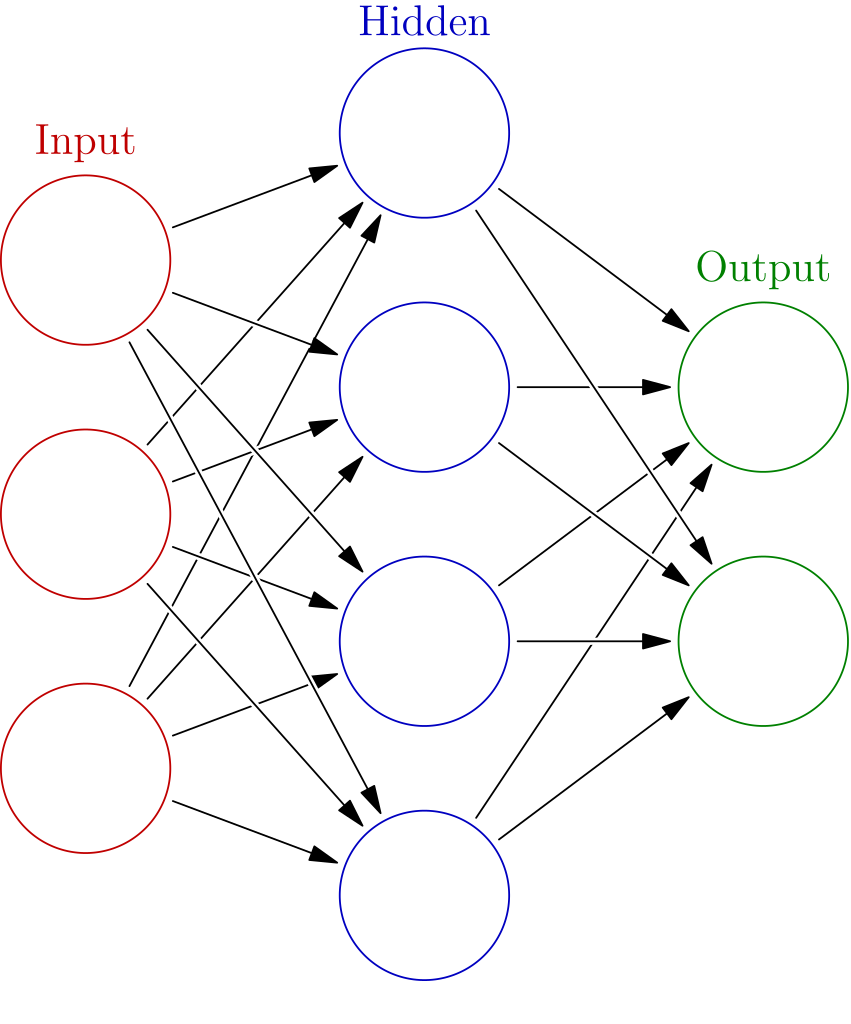
\includegraphics[width=0.3\linewidth]{figs/colored_neural_network.png}
    \caption{A schematic of a neural network with a input layer with three nodes, one hidden layer with four nodes, and an output layer with two nodes~\cite{commons_filecolored_2025}.}
    \label{fig:enter-label}
\end{figure}

Each node takes a biased weighted sum of the values of the previous layer, applies an activation function $f_a$, and outputs the value to the next layer.
\begin{equation}
    a^{(l)}_j = f_a\left(b_j^{(l)} + \sum_i w_{ij}^{(l-1)} a_i^{(l-1)}\right)
\end{equation}
Or, using matrix notation, where we define $f_a$ to act component-wise on a vector,
\begin{equation}
    \mathbf{a}^{(l)} = f_a\left(\mathbf{b}^{(l)} + \mathbf{W}^{(l-1)}\mathbf{a}^{(l-1)}\right).
\end{equation}
In this article, we will use the notation $a^{(l)}_i$ to refer to the output of node $i$ in layer $l$, and $\mathbf{a}^{(l)}$ to refer to the vector of outputs of all nodes in layer $l$. The weights and biases applied onto nodes from layer $l$ to be inputted into layer $l+1$ will be denoted as $\mathbf{W}^{(l)}$ and $\mathbf{b}^{(l)}$, respectively. Note that this superscript notation is different from the one we use with $\boldsymbol{\theta}$, which is used to denote the iteration of the gradient descent algorithm.

\subsection{Activation Functions and the Universal Approximation Theorems}

For virtually all non-trivial problems, linear relationships are far too reductive to completely capture the complexity of the task at hand. Therefore, a variety of non-linear \textbf{activation functions} are applied at each node to eliminate this kind of model bias to allow the model to learn more non-linear relationships.

\textbf{Sigmoid functions} are ubiquitous in this role, and they are also useful since they normalize the output of a node to be between $0$ and $1$. This is useful for many applications, such as when the output of a node is interpreted as a probability.
\begin{equation}
    \sigma(x) = \frac{1}{1+e^{-x}}
\end{equation}
Another very common activation function is the \textbf{\gls{relu}}, which has the advantage of being computationally easier to calculate.
\begin{equation}
    \text{ReLU}(x) = \max(0,x)
\end{equation}
\begin{figure}[h]
    \centering
    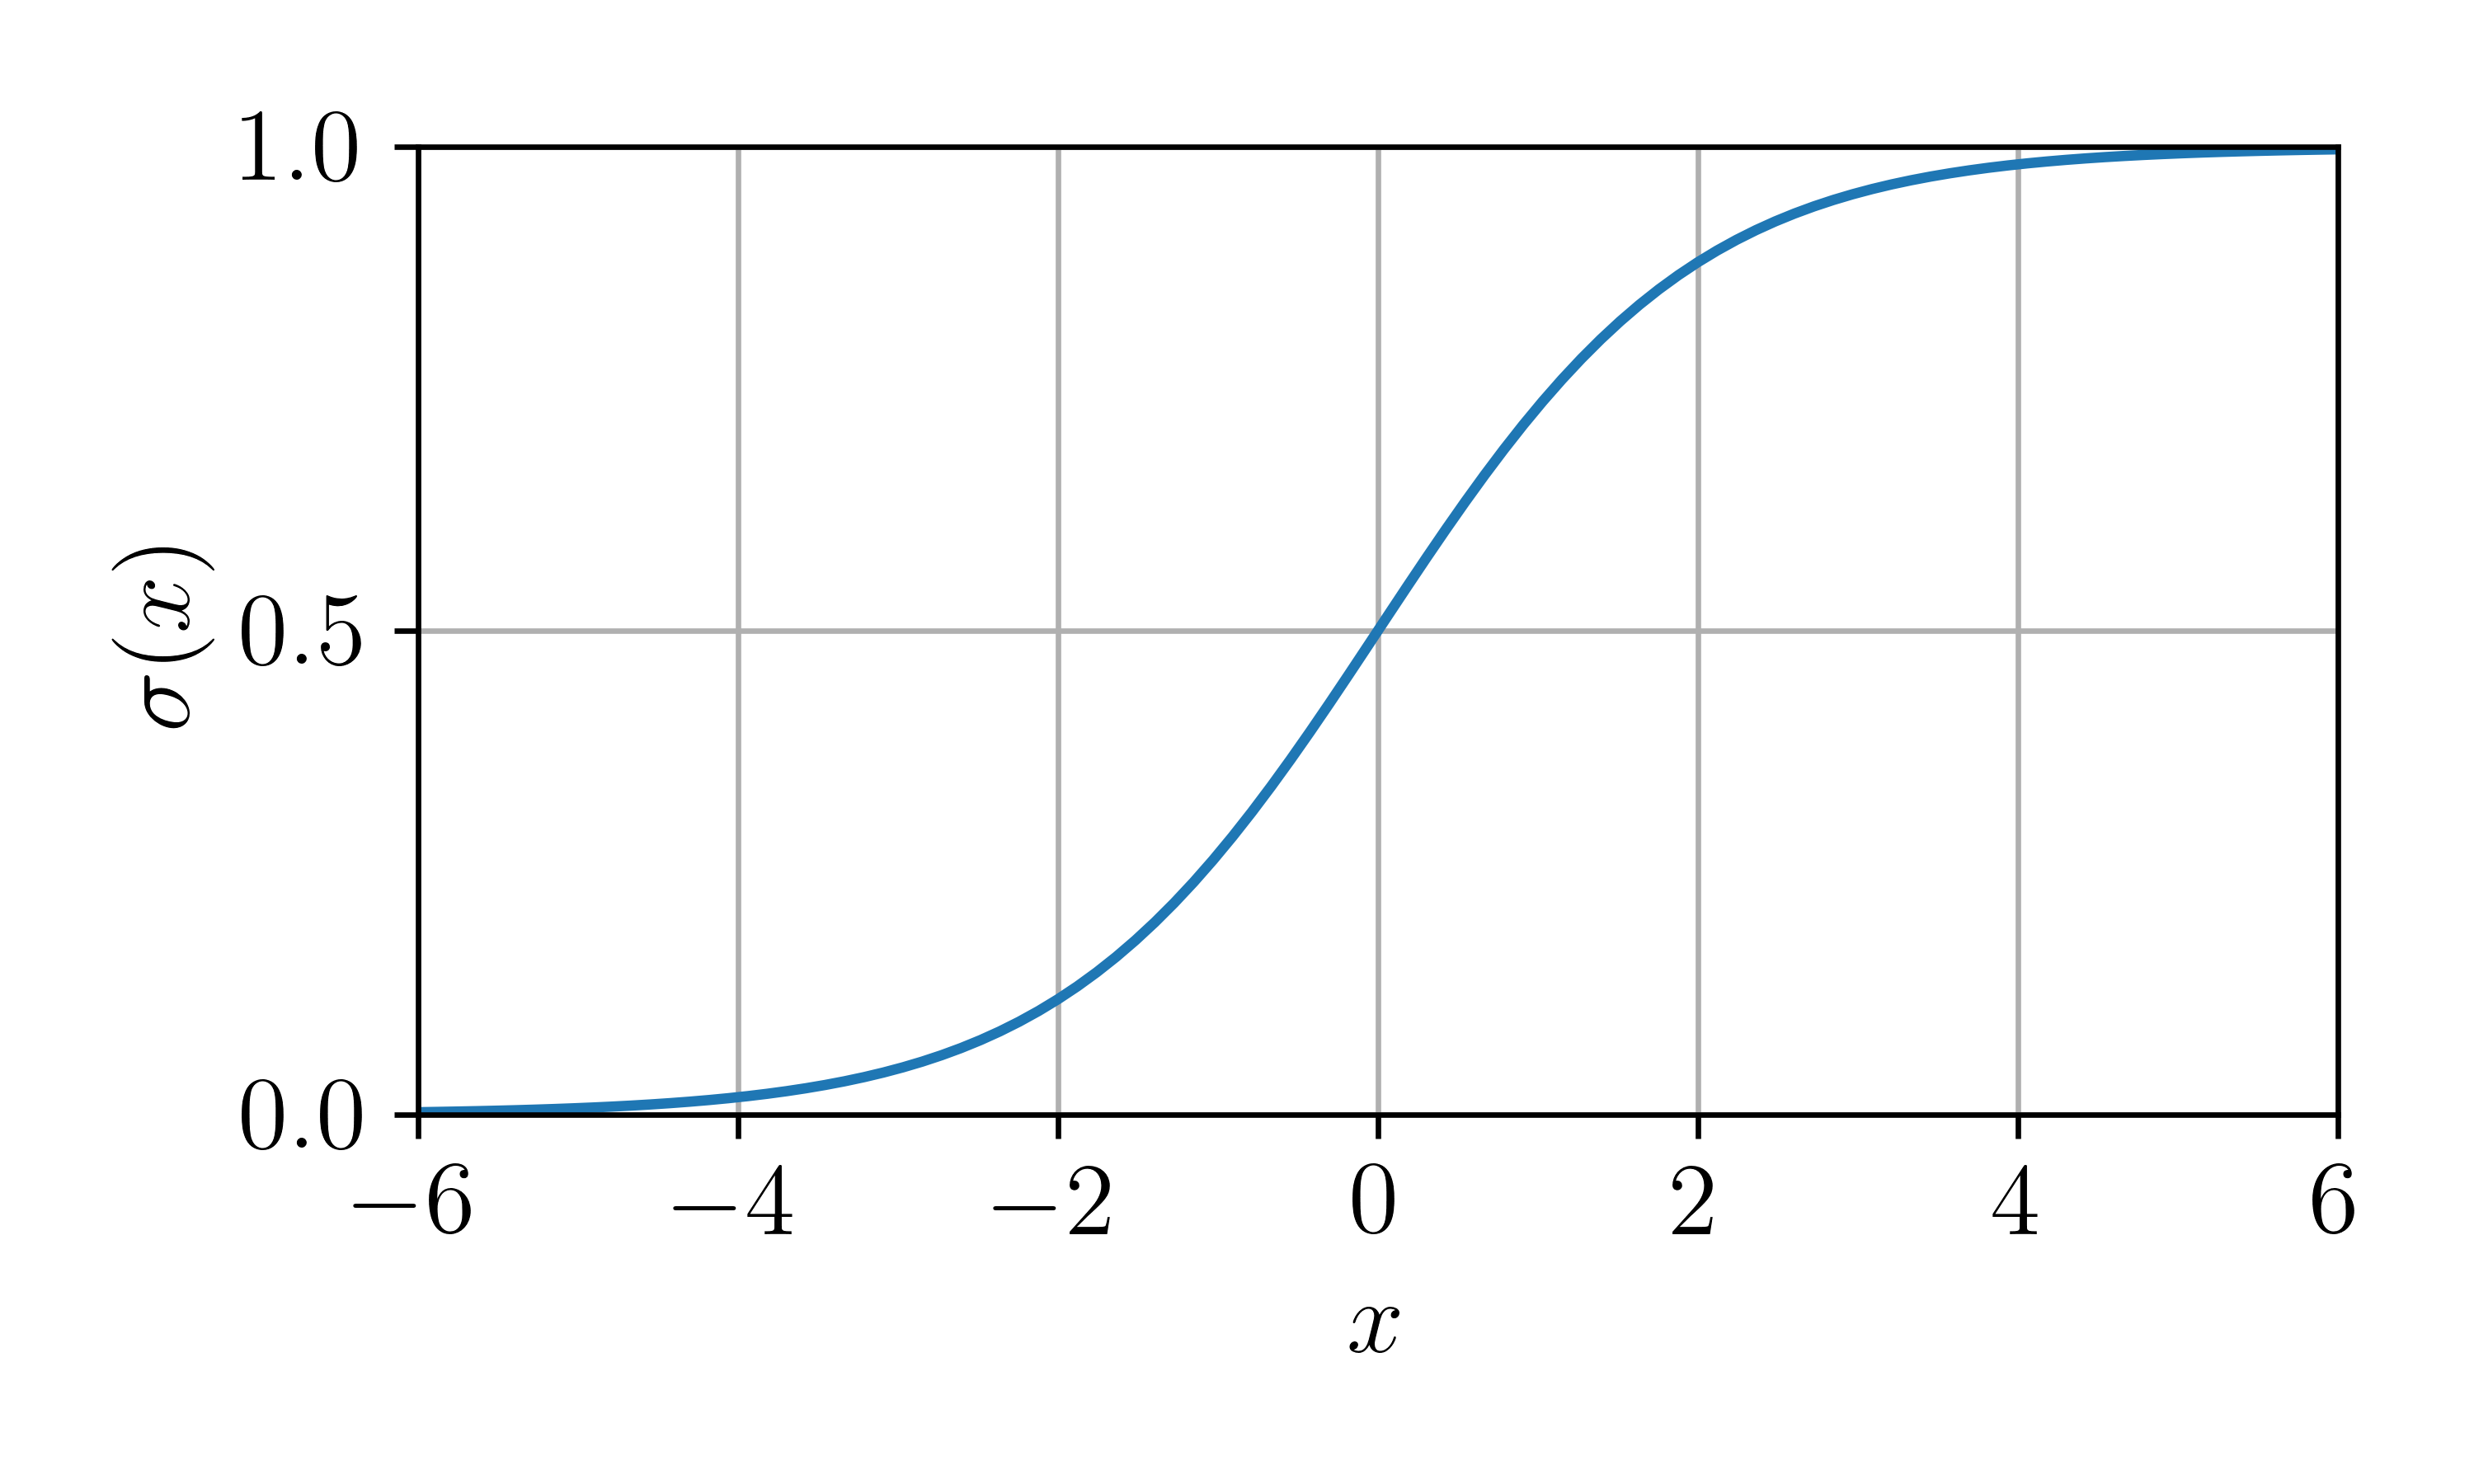
\includegraphics[width=0.45\linewidth]{figs/sigmoid.png}
    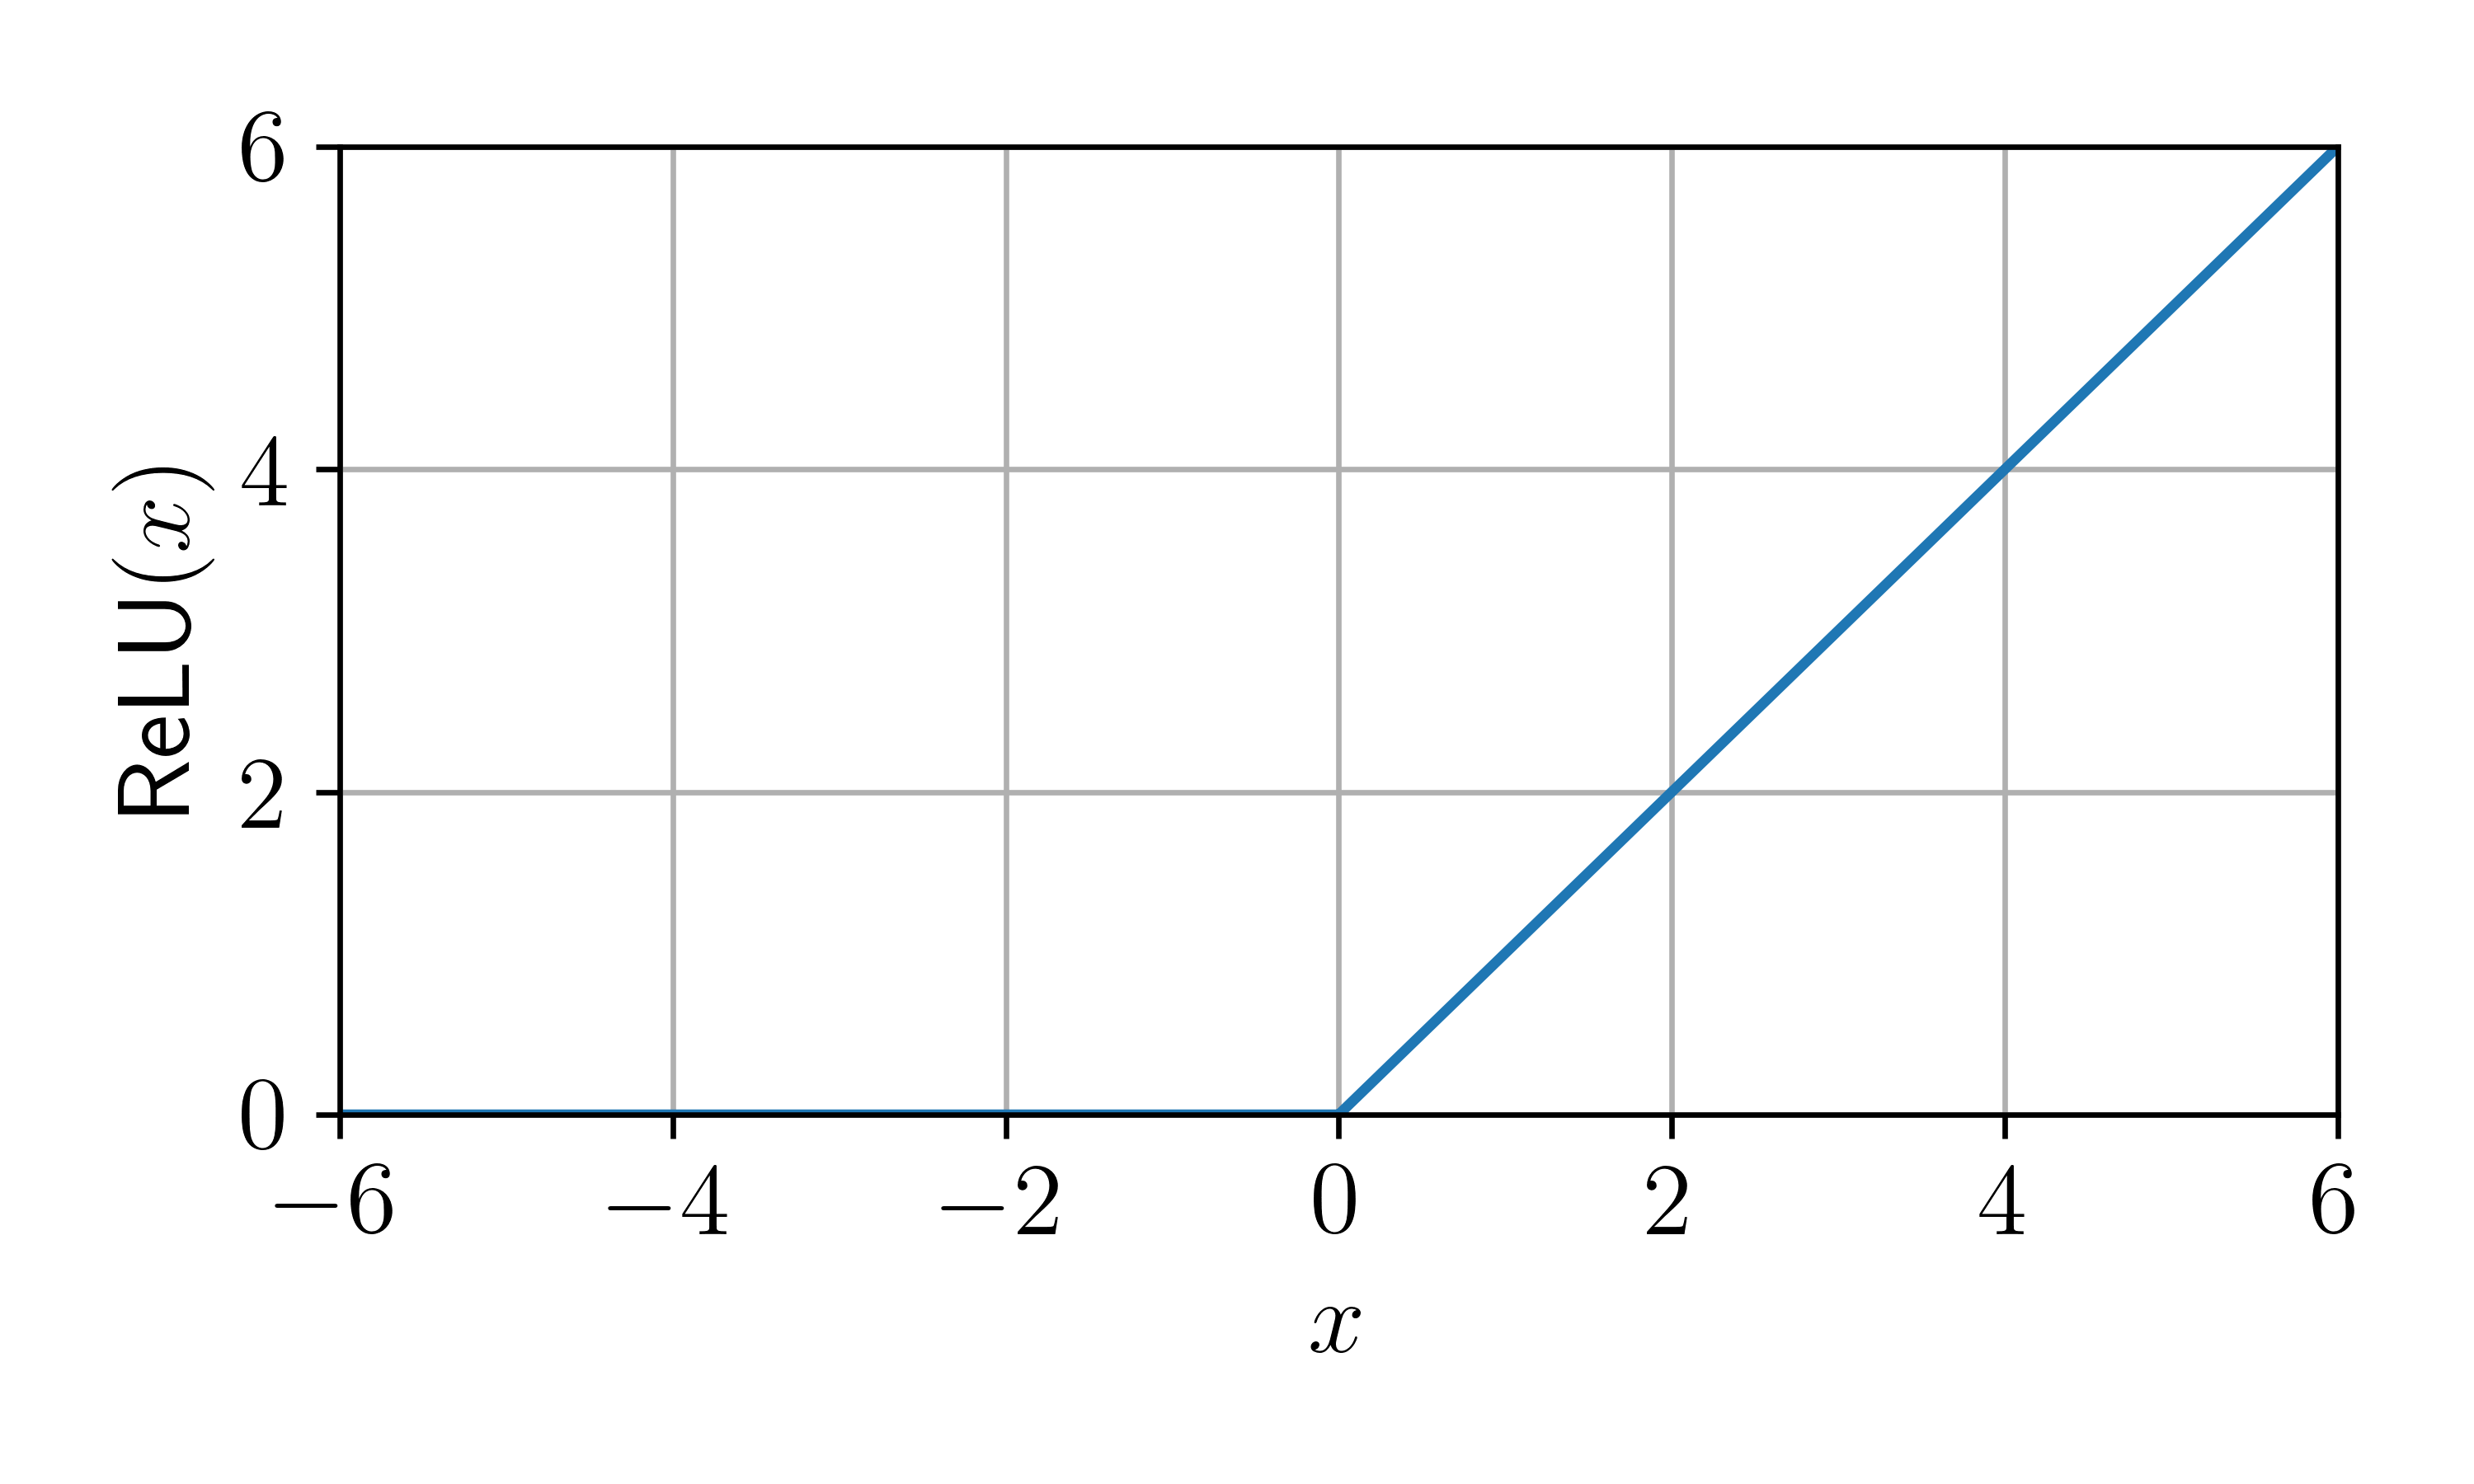
\includegraphics[width=0.45\linewidth]{figs/relu.png}
    \caption{Plot of $\sigma(x)$ (left) and $\text{ReLU}(x)$ (right). (Original)}
    \label{fig:enter-label}
\end{figure}

Any continuous relationship between two variables can be approximated by a \textit{sufficiently large} linear combination of sigmoid functions~\cite{cybenko_approximation_1989}.
\begin{equation} \label{eq:approximation}
    f \approx b + \mathbf{c} \cdot \sigma(\mathbf{b} + \mathbf{W}\mathbf{x}).
\end{equation}
Equation \ref{eq:approximation} is equivalent to a neural network with one hidden layer and scalar output (omitting the final application of an activation function).
\begin{figure}[h]
    \centering
    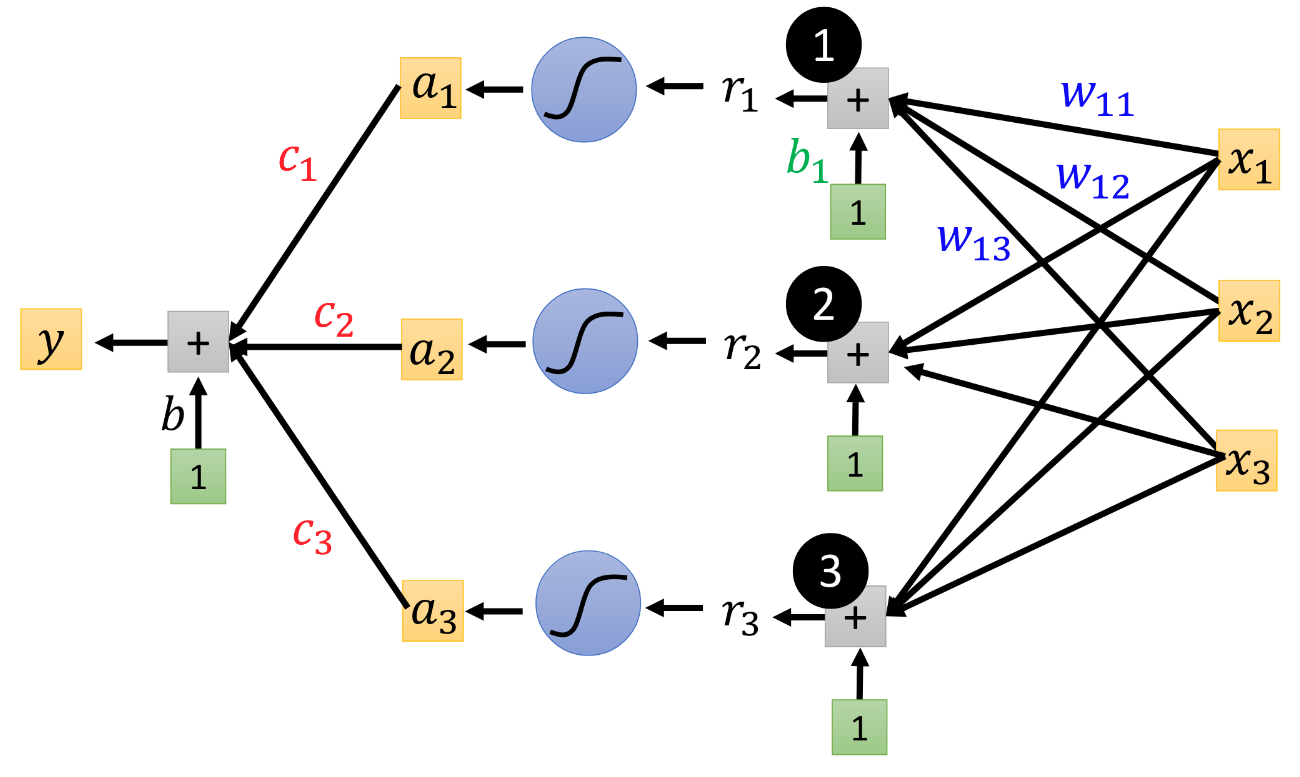
\includegraphics[width=0.5\linewidth]{figs/simple.png}
    \caption{}
    \label{fig:enter-label}
\end{figure}

This result can be generalized to any non-polynomial function, such as ReLUs, in the \textbf{universal approximation theorems}, implying that NNs that use such activation functions may theoretically learn any relationship given \textit{sufficiently large} amounts nodes and layers~\cite{hornik_multilayer_1989, kidger_universal_2020, pinkus_approximation_1999}. It is important to note that this result is only theoretical, and in practice, computational and data constraints usually frustrate this ideal.

\subsection{Layers}

The addition of layers to a model increases its complexity, the number of which is referred to as its \textbf{depth}. The number of nodes in a layer is referred to as the layer's \textbf{width}. The width and depth of a model are hyperparameters, and there is a balance to be made between model bias, computational demands, and overfitting, a phenomenon we will discuss in Section~\ref{sec:overfitting}.
\section{Backpropagation}

\textbf{Backpropagation} is the textbook algorithm for computing the gradient of the loss function. Essentially, it is the application of the chain rule to neural networks.
\begin{equation}
    \nabla L = \frac{\partial L}{\partial \theta_i} = \frac{\partial L}{\partial a_j} \frac{\partial a_j}{\partial z_j} \frac{\partial z_j}{\partial \theta_i}
\end{equation}

\section{Overfitting}\label{sec:overfitting}
\textbf{Overfitting} is a phenomenon that occurs when a model learns the training data too well, and is unable to generalize to new data. Generally, models with more parameters and degrees of freedom are more prone to overfitting. This may be mitigated by simply using a smaller model or by stopping training earlier, but these methods are not always feasible.

\subsection{Cross-validation}


\subsection{Regularization}

\subsection{Dropout}

\section{Techniques for Improving Optimization with Gradient Descent}

\subsection{Data Batching}

\subsection{Stochastic Gradient Descent}

\subsection{Momentum}

\subsection{Adaptive Learning Rate}

\subsection{Adaptive Moment Estimation (Adam)}


\section{Reinforcement Learning}

\chapter{Robotic Systems}

\section{ANYmal by ANYbotics}

\chapter{Literature}

\printglossaries

\printbibliography
\addcontentsline{toc}{chapter}{Bibliography}

\end{document}